\documentclass{letter}

\usepackage{amsmath}
\usepackage{graphicx}
\usepackage{pdfpages}

\DeclareGraphicsExtensions{.pdf, .png, .jpg}

\begin{document}

Alexandra Anderson(aea84) \\
CS 4620: a6-Animation \\
Written Questions \\

1. 

a. 
\begin{align*}
& M_0 = 
\begin{pmatrix}
0.5 & 0 \\
0 & 1.5
\end{pmatrix}
\quad \quad 
& M_1 = 
\begin{pmatrix} 
0 & 1.5 \\ 
-0.5 & 0
\end{pmatrix} \\
& M_{0.5}^{lin} = 
\begin{pmatrix}
0.25 & 0.75 \\
-0.25 & 0.75
\end{pmatrix} \\
& R_0 = 
\begin{pmatrix}
1 & 0 \\
0 & 1
\end{pmatrix}
\quad \quad 
& S_0 = 
\begin{pmatrix}
0.5 & 0 \\
0 & 1.5
\end{pmatrix} \\
& R_1 = 
\begin{pmatrix}
0 & 1 \\
-1 & 0
\end{pmatrix}
\quad \quad 
& S_1 = 
\begin{pmatrix}
0.5 & 0 \\
0 & 1.5
\end{pmatrix} \\
& R_{0.5} = 
\frac{1}{\sqrt{2}}
\begin{pmatrix}
1 & 1 \\
-1 & 1
\end{pmatrix}
& S_{0.5} = 
\frac{1}{2}
\begin{pmatrix}
1 & 0 \\
0 & 3
\end{pmatrix} \\
& M_{0.5}^{pol} =
\frac{1}{2\sqrt{2}}
\begin{pmatrix}
1 & 1 \\
-1 & 3
\end{pmatrix} 
\end{align*}

b. 

We observe that $M_0$ and $M_1$ can easily be written as a composition $SR$, where $S$ is a scale of x=0.5 and y=1.5, and where $R$ is a rotation 45 degrees clockwise or counter-clockwise. Calculations follow from this premise. 

\begin{align*} 
& M_0 = 
\frac{1}{2\sqrt{2}}
\begin{pmatrix}
1 & -1 \\
3 & 3 
\end{pmatrix} 
\quad \quad 
& M_1 = 
\frac{1}{2\sqrt{2}}
\begin{pmatrix} 
1 & 1 \\
-3 & 3 
\end{pmatrix} \\
& M_{0.5}^{lin} = 
\frac{1}{2\sqrt{2}} 
\begin{pmatrix} 
1 & 0 \\
0 & 3
\end{pmatrix} \\
\end{align*}

We calculate the polar decomposition by noting that $R = M^TS$, where $S$ is symmetric. Thus, we derive (in lecture) that $(s, c) = norm(m_{21} - m_{12}, m_{11} + m_{22})$. For $M_0$, the un-normalized vector is $(m_{21} - m_{12}, m_{11} + m_{22}) = (\sqrt{2}, \sqrt{2})$, and the normalization is $(\frac{1}{\sqrt{2}}, \frac{1}{\sqrt{2}})$. This gives us the value of $R$, and $S$ is easily computable from there. 

For $M_1$, our key vector is $(m_{21} - m_{12}, m_{11} + m_{22}) = (-\sqrt{2}, \sqrt{2})$, and it normalizes to $(-\frac{1}{\sqrt{2}}, \frac{1}{\sqrt{2}})$. 

\begin{align*} 
& R_0 = 
\frac{1}{\sqrt{2}}
\begin{pmatrix}
1 & -1\\
1 & 1
\end{pmatrix} \\
\quad \quad
& S_0 = 
\frac{1}{2}
\begin{pmatrix}
2 & 1 \\
1 & 2
\end{pmatrix} \\
& R_1 = 
\frac{1}{\sqrt{2}} 
\begin{pmatrix}
1 & 1 \\
-1 & 1
\end{pmatrix}
\quad \quad 
& S_1 = 
\frac{1}{2}
\begin{pmatrix}
2 & -1 \\
-1 & 2
\end{pmatrix} \\ 
& R_{0.5} = 
\begin{pmatrix}
1 & 0 \\
0 & 1
\end{pmatrix}
& S_{0.5} = 
\begin{pmatrix} 
1 & 0 \\
0 & 1
\end{pmatrix} \\
& M_{0.5}^{pol} = 
\begin{pmatrix}
1 & 0 \\
0 & 1
\end{pmatrix} 
\end{align*}

c. 
\begin{align*} 
& M_0 = 
\frac{1}{2\sqrt{2}}
\begin{pmatrix}
1 & -1 \\
3 & 3 
\end{pmatrix}
\quad \quad 
& M_1 = 
\frac{1}{2\sqrt{2}}
\begin{pmatrix} 
3 & 3  \\ 
-1  & 1
\end{pmatrix} \\
& M_{0.5}^{lin} = 
\frac{1}{2\sqrt{2}}
\begin{pmatrix}
2 & 1\\
1 & 2
\end{pmatrix} \\
\end{align*}

We calculate our polar decomposition again. For $M_0$, the vector is $(m_{21} - m_{12}, m_{11} + m_{22}) = (\frac{2}{\sqrt{2}}, \frac{2}{\sqrt{2}})$, which normalizes to $(\frac{1}{\sqrt{2}}, \frac{1}{\sqrt{2}})$. 

For $M_1$, the vector is $(m_{21} - m_{12}, m_{11} + m_{22}) = (-\frac{2}{\sqrt{2}}, \frac{2}{\sqrt{2}})$, which again normalizes to $(-\frac{1}{\sqrt{2}}, \frac{1}{\sqrt{2}})$.

\begin{align*}
& R_0 = 
\frac{1}{\sqrt{2}}
\begin{pmatrix}
1 & -1 \\ 
1 & 1
\end{pmatrix}
\quad \quad 
& S_0 = 
\frac{1}{2}
\begin{pmatrix}
2 & 1 \\
1 & 2
\end{pmatrix} \\
& R_1 = 
\frac{1}{\sqrt{2}}
\begin{pmatrix} 
1 & 1 \\
-1 & 1
\end{pmatrix}
\quad \quad 
& S_1 = 
\frac{1}{2}
\begin{pmatrix}
2 & 1 \\
1 & 2
\end{pmatrix} \\
& R_{0.5} =  
\begin{pmatrix}
1 & 0 \\
0 & 1
\end{pmatrix}
& S_{0.5} = 
\frac{1}{2}
\begin{pmatrix}
2 & 1 \\
1 & 2
\end{pmatrix} \\
& M_{0.5}^{pol} =
\begin{pmatrix}
1 & 0.5 \\
0.5 & 1
\end{pmatrix} 
\end{align*}

(Graphs)

On the following pages are graphs. The first page has linear interpolations for a, b, and c. The second page has polar interpretations for a, b, and c. 

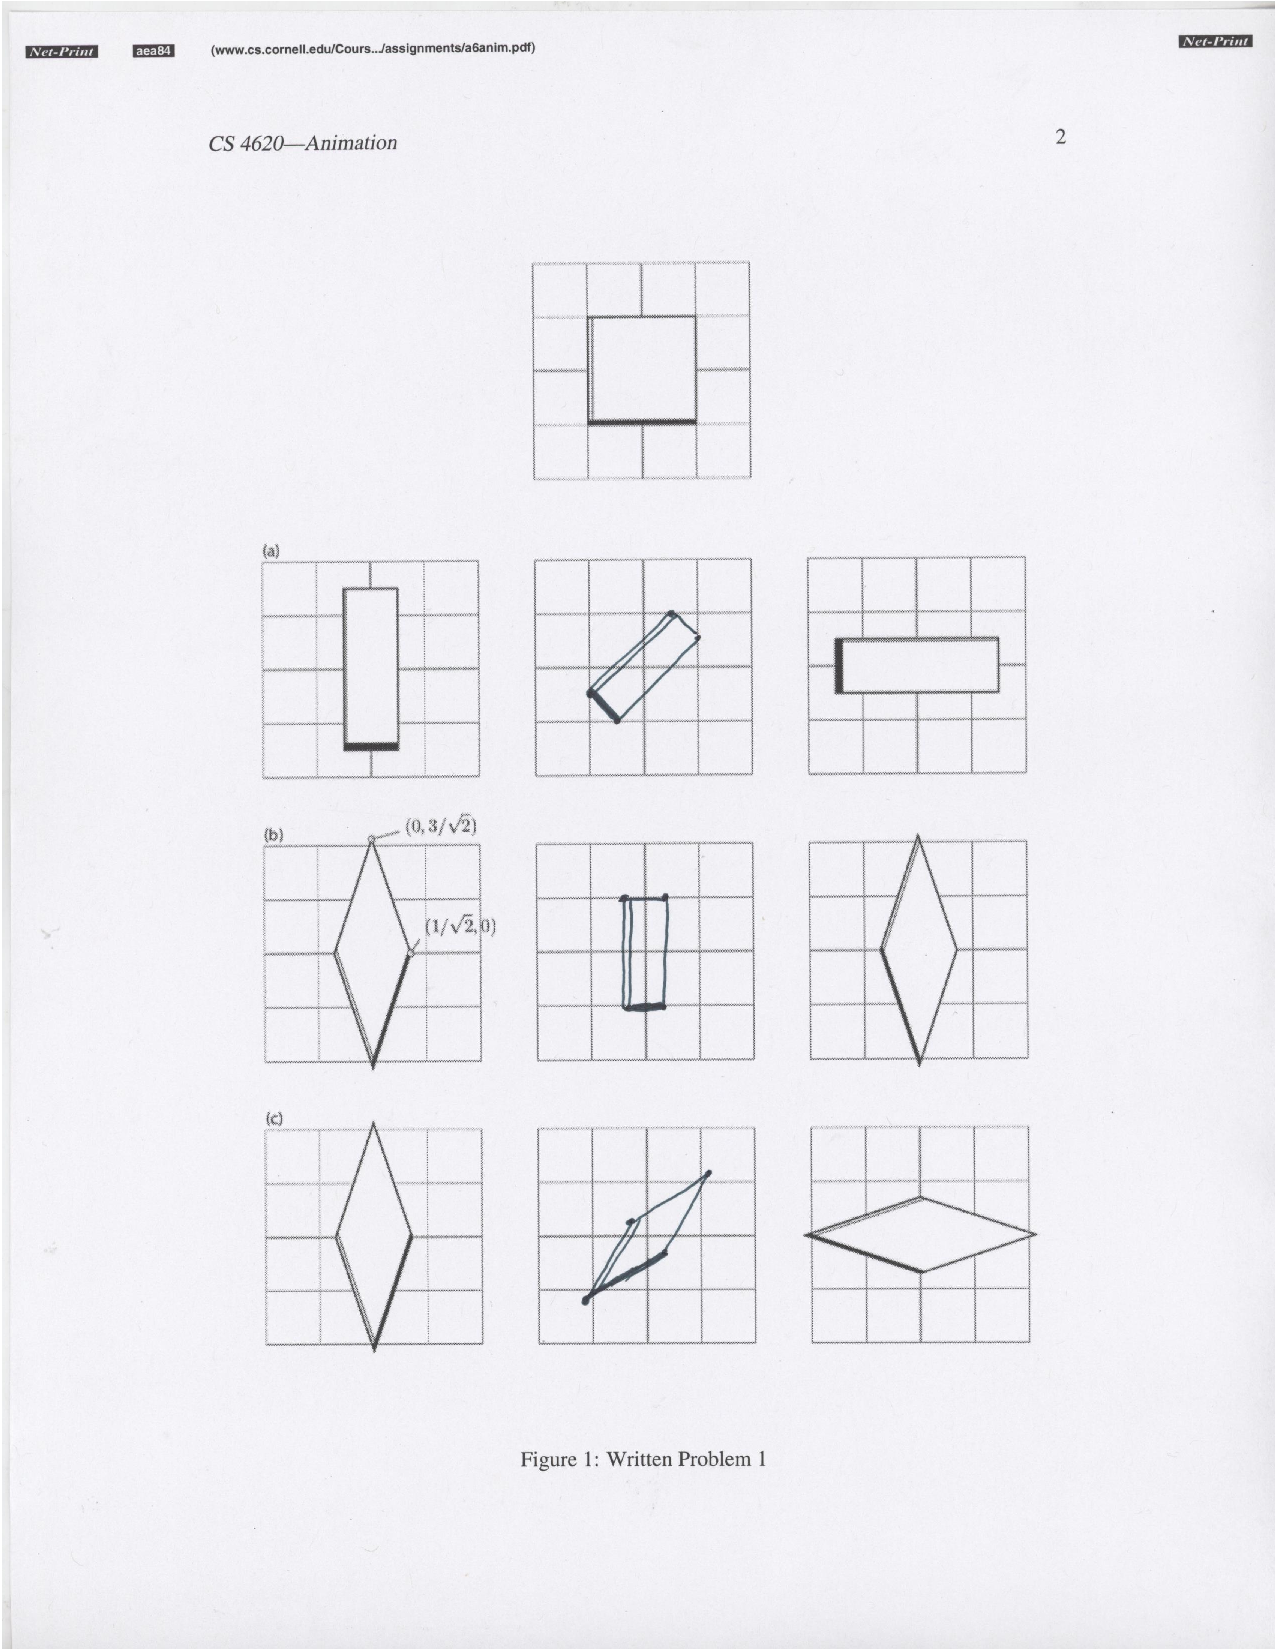
\includepdf{linear}

 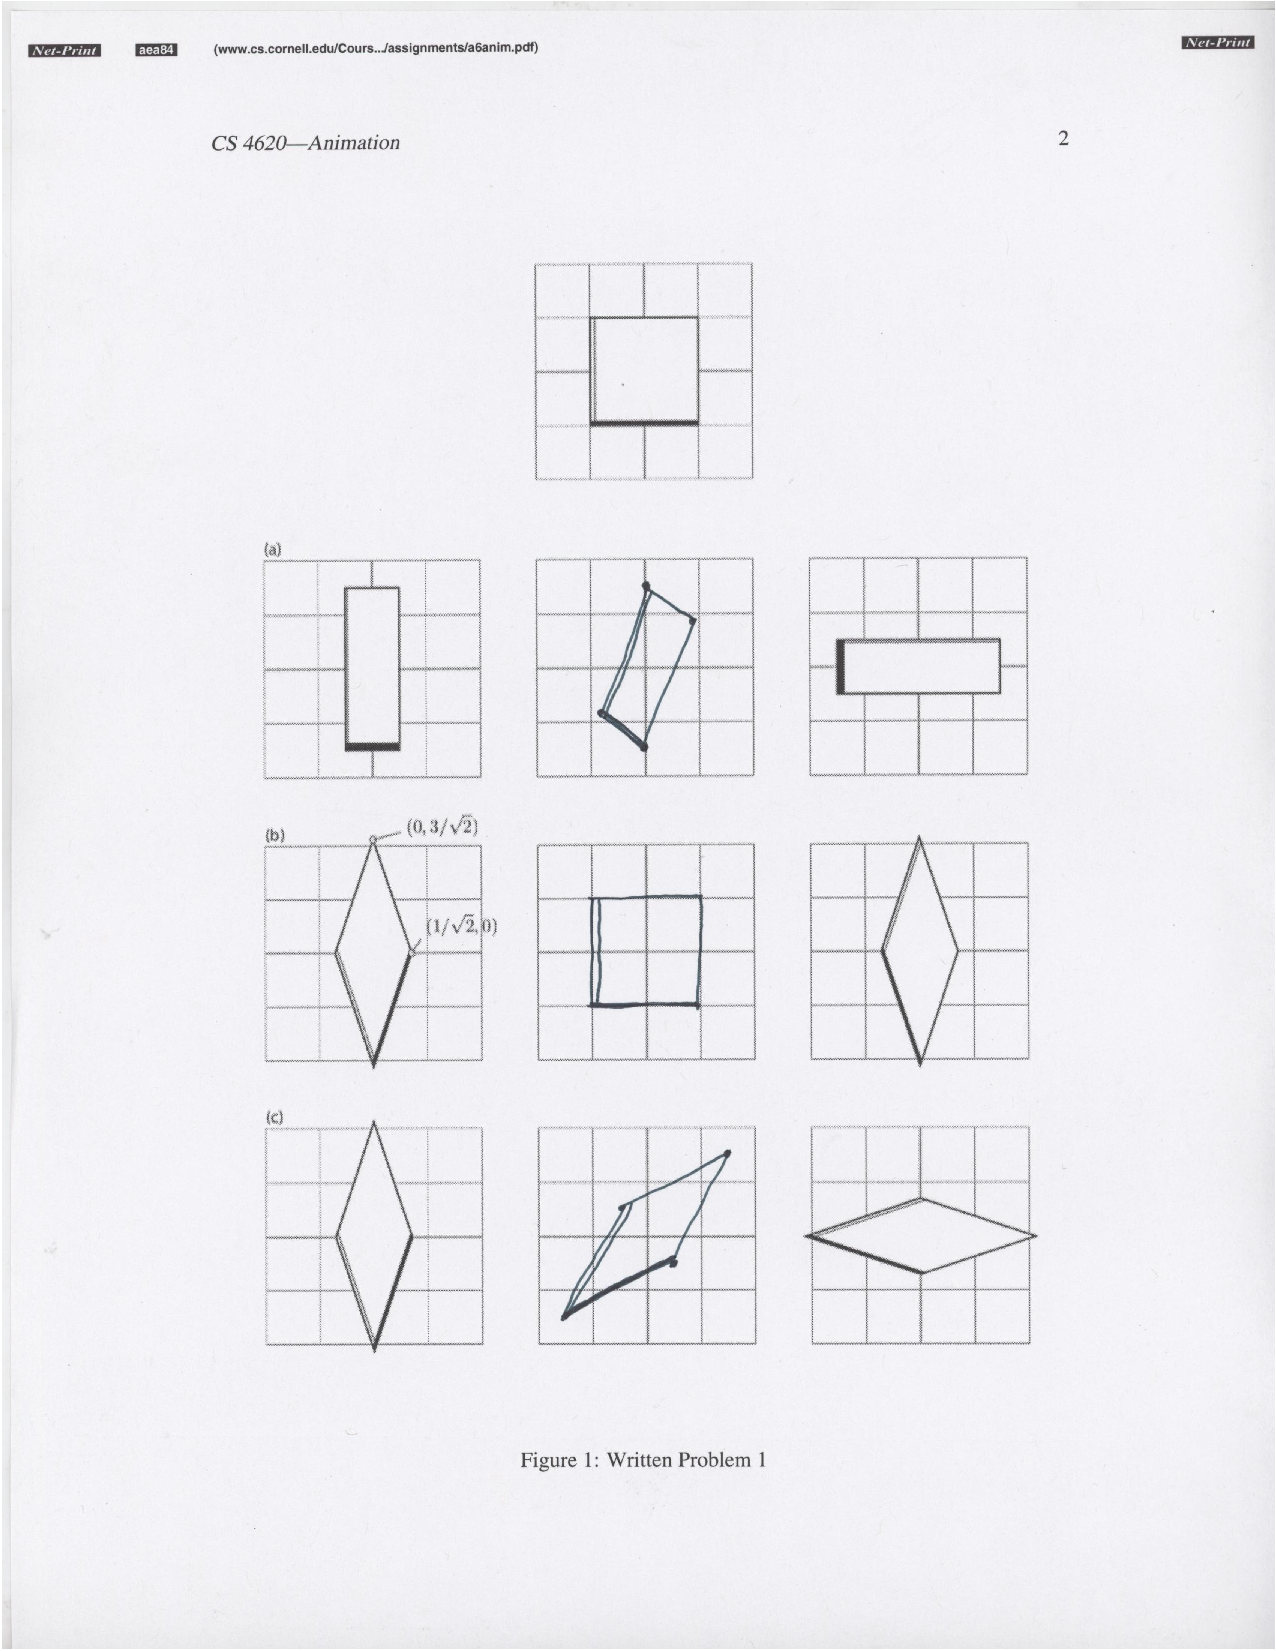
\includepdf{polar}

2. 

1. 
Rotation of 0 degrees around the X-axis : (1, 0, 0, 0)
Rotation of 180 degrees around the X-axis : (0, 1, 0, 0)

2.
Their spherical interpolation one-quarter of the way is : $(-0.5411961, 1.3065629, -0.5411961, 1.3065629)$, which corresponds to 45 degrees around the X-axis. 

3.
We convert $(0, \sqrt{2}, 0, \sqrt{2})$ to a 3x3 matrix:
$$\begin{pmatrix}
0 & 0 & 1 \\
-\frac{1}{\sqrt{2}} & -\frac{1}{\sqrt{2}} & 0 \\
\frac{1}{\sqrt{2}} & -\frac{1}{\sqrt{2}} & 0 \\
\end{pmatrix}$$

Yes, this is the matrix that would be generated for 45-degrees around the x-axis. 

4. The matrix for a x-rotation of 90 degrees followed by a y-rotation of 90 degrees is :
$$\begin{pmatrix}
0 & 1 & 0 \\
0 & 0 & -1 \\
-1 & 0 & 0 \\
\end{pmatrix}$$
Its quaternion is $q_4 = (0.5, 0.5, 0.5, -0.5)$.

The  matrix for a y-rotation of 90 degrees followed by a z-rotation of 90 degrees is :
$$\begin{pmatrix}
0 & -1 & 0 \\
0 & 0 & 1 \\
-1 & 0 & 0 \\
\end{pmatrix}$$
Its quaternion is $q_5 = (-0.5, 0.5, -0.5, -0.5)$.

5. $q_6 = (0, 0.7653668, -1.847759, 0)$. This corresponds to the axis (0.67859834, -0.28108466, -0.67859834) and angle 1.2967819 in radians, or ~74 degrees.

6. $q_7$, the rotation from $q_4$ to $q_6$, is (-0.38268343, 0.0, 0.0, 0.92387956). 

7. $q_7$ corresponds to the axis (0.0, 0.0, 1.0) and angle 1.1780974 radians. 


\end{document}